\documentclass[a4paper, 12pt]{report}

\usepackage{alltt, fancyvrb, url}
\usepackage{graphicx}
\usepackage[utf8]{inputenc}
\usepackage{float}
\usepackage{hyperref}
\usepackage{xurl}

\usepackage[italian]{babel}
\usepackage[italian]{cleveref}
\usepackage[toc,page]{appendix}

\title{Relazione Progetto Programmazione di Reti 2022}
\author{Michele Montesi \\
        Matricola: 0000974934 \\
        E-Mail: michele.montesi3@studio.unibo.it}
\date{\today}

\begin{document}

\maketitle
\tableofcontents

\chapter{Analisi}
Si é realizzata la traccia numero 2, la quale riguarda la creazione di un'architettura
\textbf{Client-Server}, utilizzando il protocollo di strato di trasporto \texttt{UDP}, per il trasferimento
di file.
Deve essere possibile lo scambio di due tipi di messaggio:
\begin{itemize}
    \item Messaggi di comando
    \item Messaggi di risposta
\end{itemize}
Le funzioni richieste sono:
\begin{itemize}
    \item \textbf{LIST}: lista dei file contenuti all'interno del server.
    \item \textbf{GET}: comando di richiesta file dal server.
    \item \textbf{PUT}: upload di un file sul server.
\end{itemize}

\chapter{Design}

\section{Panoramica}

\begin{figure}[H]
    \centering
    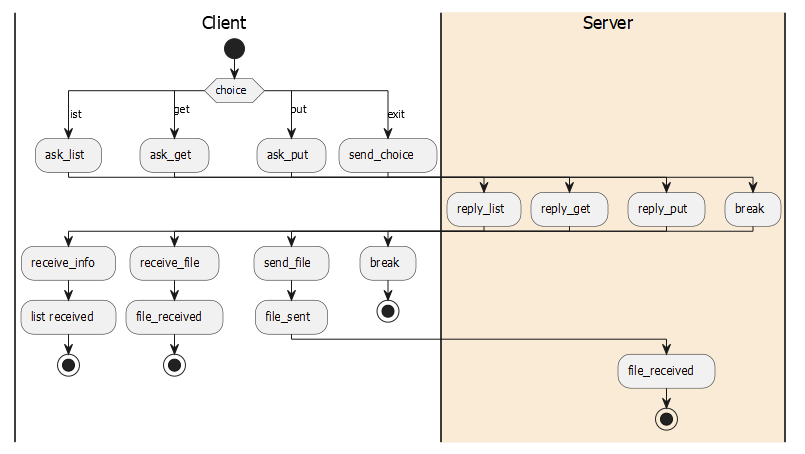
\includegraphics[width=10cm]{img/funzionamento.png}
    \caption{Rappresentazione minimale funzionamento Client Server}
\end{figure}

L'architettura é composta da due moduli: il modulo lato \texttt{client} ed il modulo lato \texttt{server}.
\begin{itemize}
    \item Per quanto riguarda il lato client, é stata implementata una classe \emph{client}, la qquale fornisce ed espone
    in console le funzionalitá richieste.
    \item Il server, sta in ascolto, aspettando un input riguardante la funzione scelta dal client.
    Quando perviene la richiesta, il server avvia un thread riguardante l'operazione in questione.
\end{itemize}
Le funzioni in comune tra i due moduli sono stati inseriti in una classe di utility evitando cosí la ripetizione del codice.

\section{Design dettagliato}
\subsection{Invio di un file da Client a Server}
Per selezionare un file verrá fatta una verifica della sua esistenza. Nel caso esista si proseguirá
con l'invio, altrimenti verrá restituito un messaggio d'errore. Appurata l'esistenza di questo, viene inviato
al server il nome del file assieme alla sua dimensione, inviando una stringa. Questa é separata da una costante \emph{Separator}
la quale sará usata come divisore tra le due informazioni. Una volta arrivata al server, questo inizierá la scrittura
di un file a cui verrá dato il nome del file originale con una \emph{'r\_'} davanti, questo permette di evitare l'\emph{overwrite} di file
originali del server ma la permette per file caricati in un primo momento, i quali devono essere aggiornati alla nuova versione.
\\
Per compiere l'operazione di \emph{put} é stato deciso di dividere il file in questione in blocchi da \(1024\) bytes.
\\
Per seguire l'andamento dell'invio del file é stata inserita una barra di progressione divisa anch'essa in blocchi da 1024 bytes.
Per completare l'invio del file verrá inviata una stringa contenente \texttt{file\_shared\_exit}.
Il server quando leggerá questa stringa tra i bytes ricevuti, interromperá la ricezione e chiuderá il socket.

\begin{figure}[H]
    \centering
    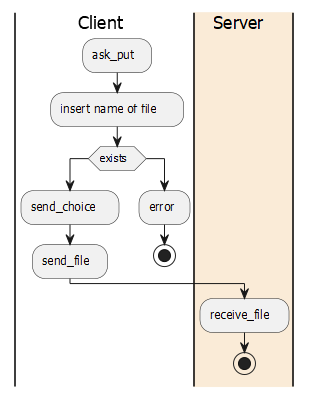
\includegraphics[height=9cm]{img/clientToServer.png}
    \caption{Invio di un file da Client a Server}
\end{figure}

\newpage
\subsection{Ricezione di un file da Server a Client}
Il meccanismo di \emph{get} é praticamente uguale al meccanismo di \emph{put} con l'unica differenza
che il controllo di esistenza del file viene eseguito sul server, il quale nel caso di esistenza
consente l'invio del file, mentre in caso contrario restituirá un messaggio d'errore.

\begin{figure}[H]
    \centering
    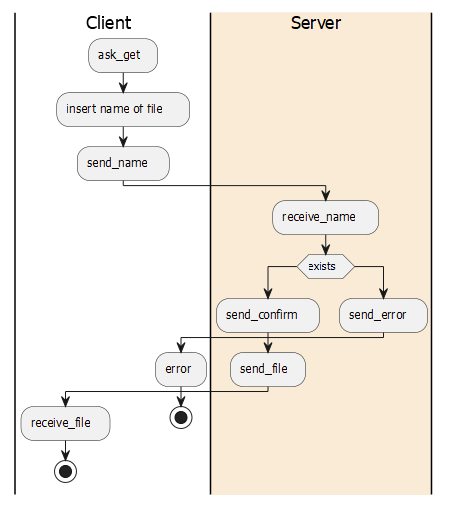
\includegraphics[height=9cm]{img/serverToClient.png}
    \caption{Invio di un file da Server a Client}
\end{figure}

\chapter{Threads attivi}
Per ogni funzione, sia lato Server che lato Client, viene avviato un Thread, in modo che il server possa comunicare
con piú client.

\section{Operazioni simultanee}
\subsubsection{Possibili}
\begin{itemize}
    \item \emph{list} + \emph{put} or \emph{get}
    \item \emph{put} + \emph{get}
\end{itemize}

\subsubsection{Non Possibili}
\begin{itemize}
    \item \emph{put} + \emph{put}
    \item \emph{get} + \emph{get}
\end{itemize}

\end{document}